Σκοπός είναι η εύρεση της τιμής της αντίστασης $R$ του κυκλώματος \ref{circ:spice:1_schematic} προκειμένου να μην υπάρχει παραμόρφωση στην έξοδο της γεννήτριας και εν συνεχεία ο προσδιορισμός της συχνότητας της κυματομορφής της εξόδου για την τιμή της $R$ που βρέθηκε.\par
Αρχικά εκτελείται parametric sweep για $1\kohm\leqslant R\leqslant 101\kohm$ με βήμα $20\kohm$. Παρατηρείται η έξοδος του κυκλώματος, $v_{\mathrm{out}}$, στο πεδίο του χρόνου στο διάστημα $\lb 0,2.05 \rb\unit{\milli\second}$. Τα αποτελέσματα φαίνονται στο διάγραμμα \ref{plot:ask1:q5_1}.

\begin{plot_fig}[H]
	\begin{center}
		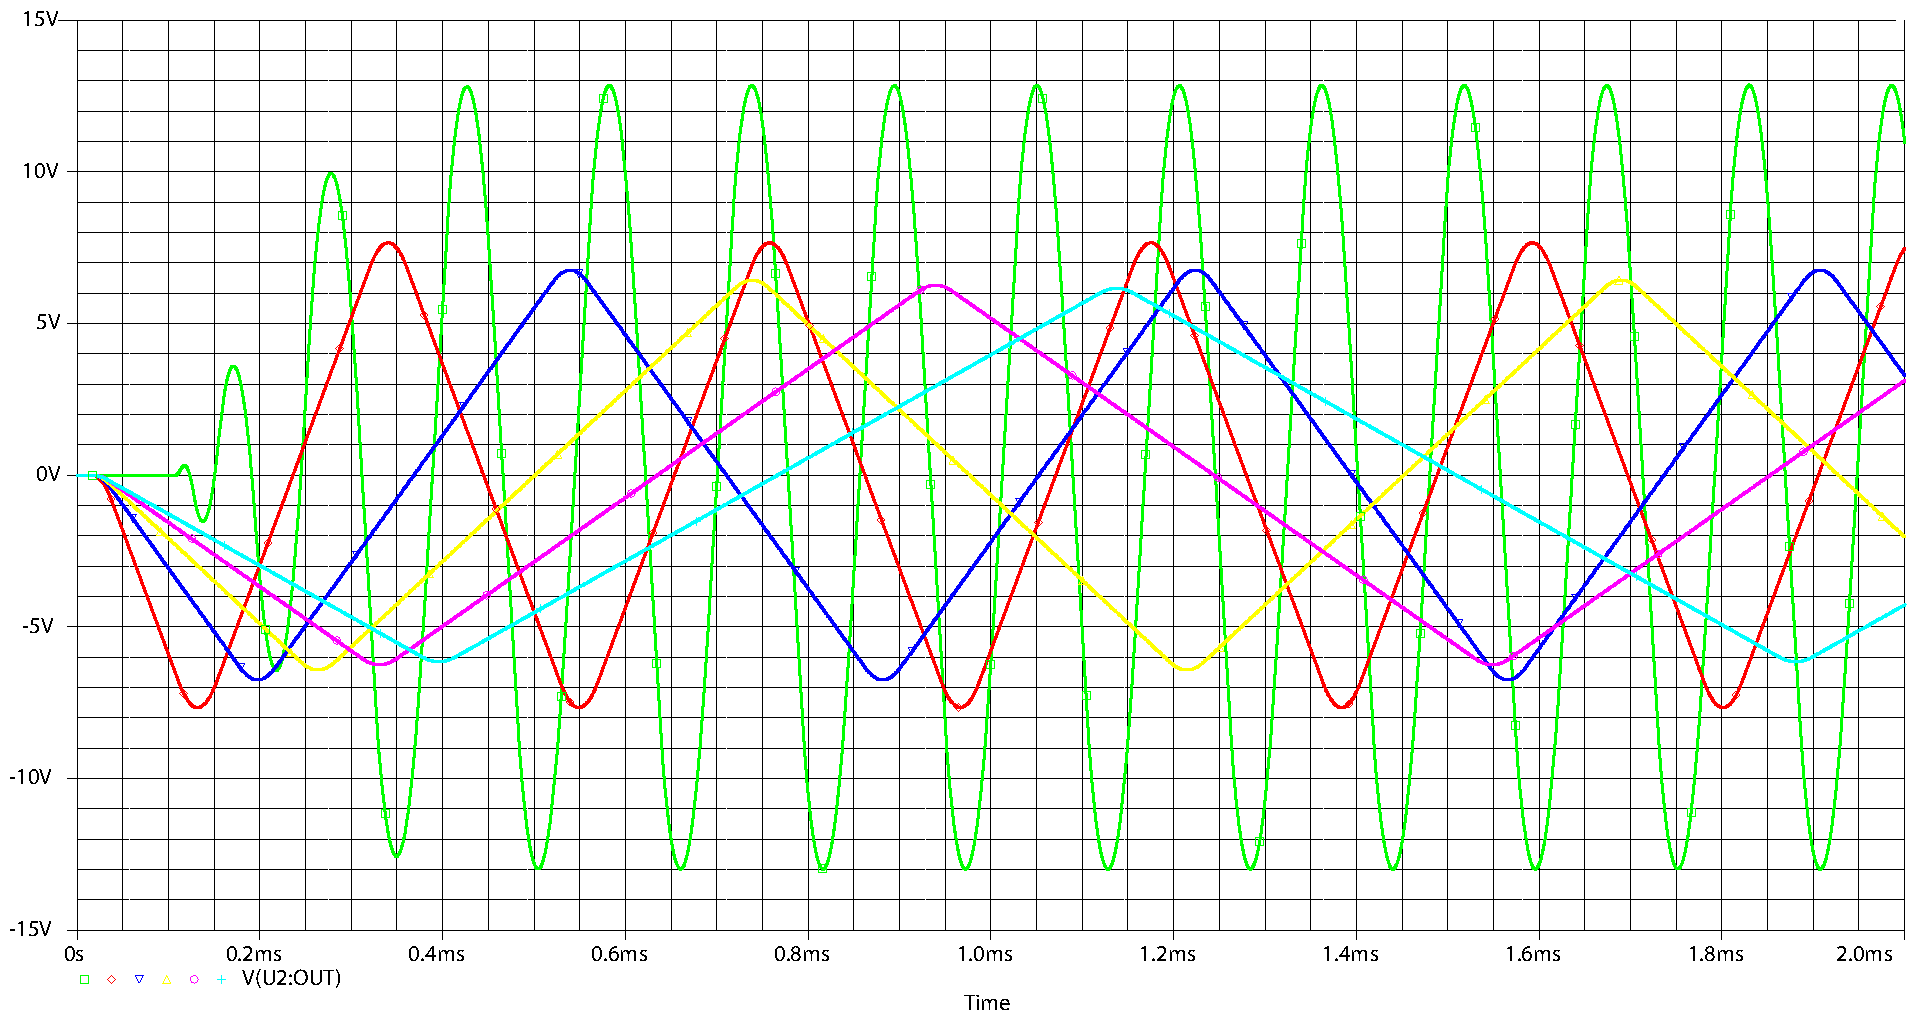
\includegraphics[width=15cm]{spice_01/q5_1.pdf}
		\caption{$v_{\mathrm{out}}$ για $R\in\left\{1,21,\ldots,101\right\}\kohm$.}
		\label{plot:ask1:q5_1}
	\end{center}
\end{plot_fig}

Στο διάγραμμα \ref{plot:ask1:q5_1} παρατηρείται παραμόρφωση της κυματομορφής $v_{\mathrm{out}}$ μόνο για την τιμή $R=1\kohm$. Επόμενο βήμα είναι η παραμετρική ανάλυση για $1\kohm\leqslant R\leqslant 18\kohm$ με βήμα $4\kohm$. Σε αντίθεση με προηγουμένως, συν της $v_{\mathrm{out}}$ παρατηρείται και η $v_2$ προκειμένου να βρεθεί με μεγαλύτερη ακρίβεια η τιμής της $R$ για την οποία υπάρχει παραμόρφωση. Τα αποτελέσματα δίδονται στο διάγραμμα \ref{plot:ask1:q5_2}.

\begin{plot_fig}[H]
	\begin{center}
		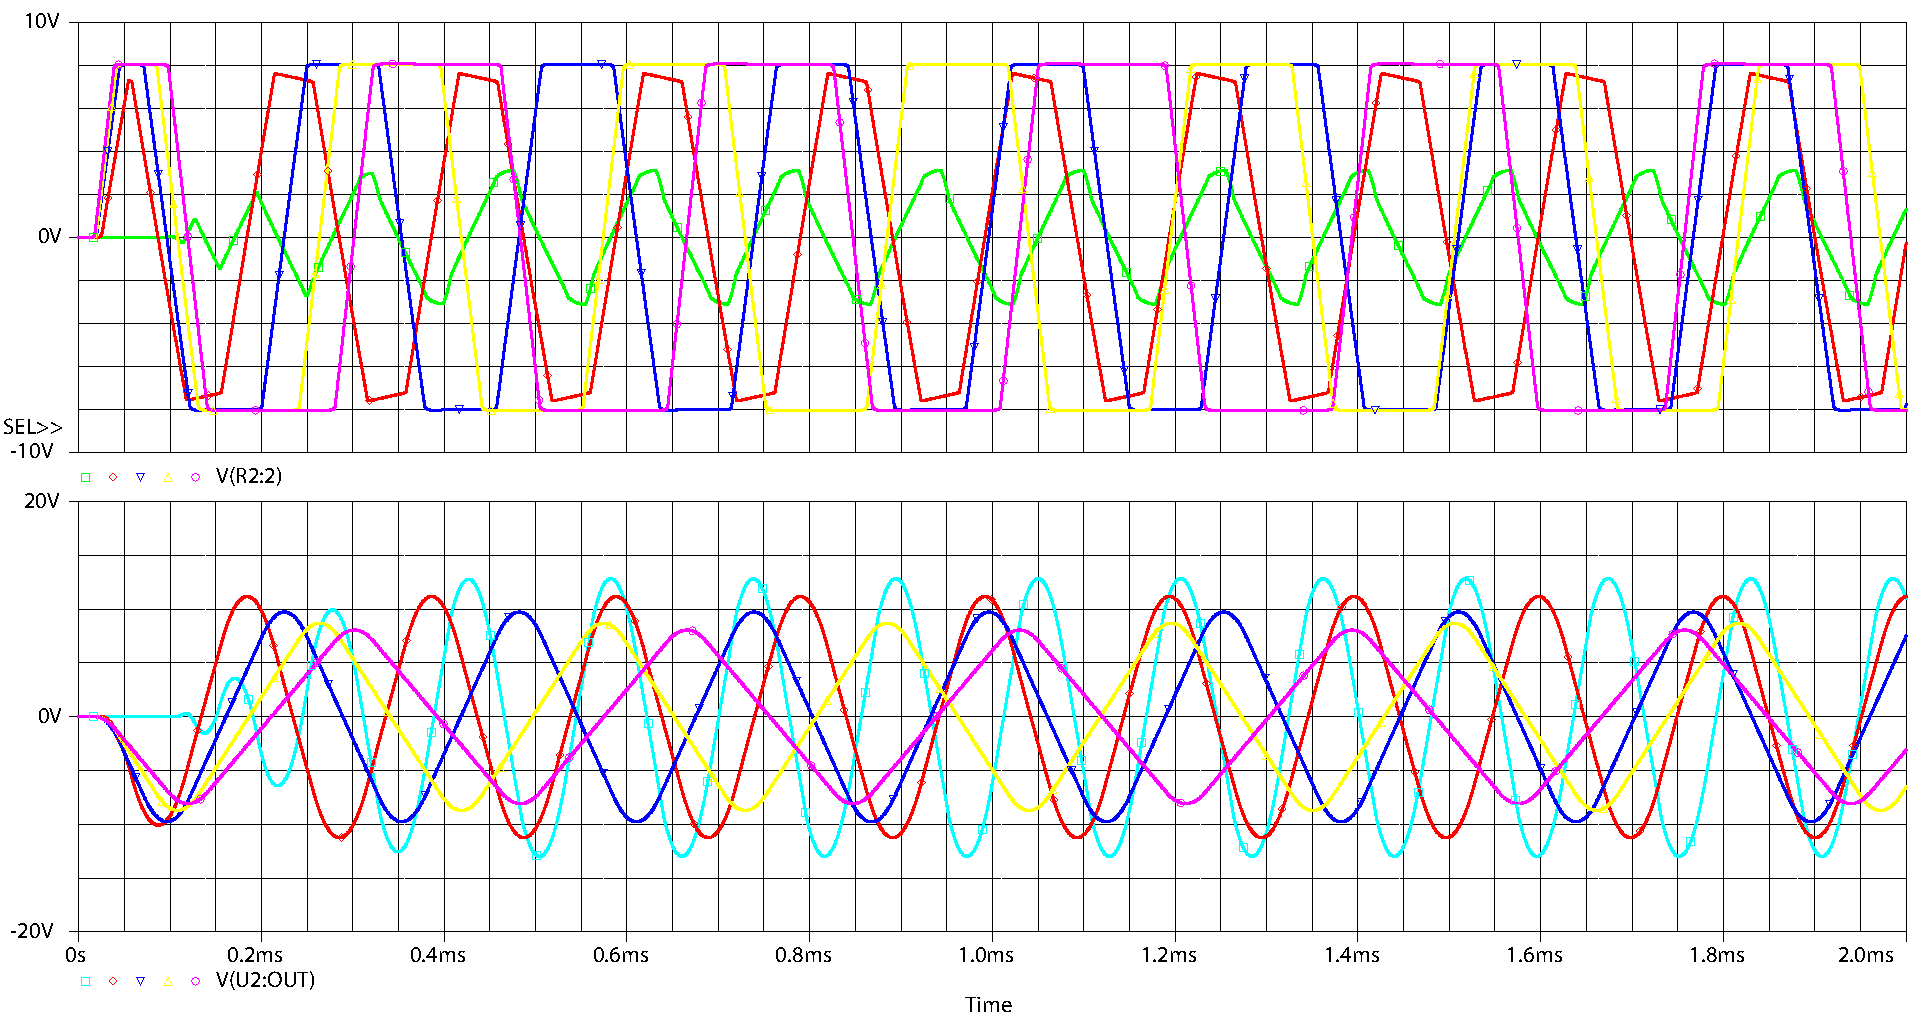
\includegraphics[width=15cm]{spice_01/q5_2.pdf}
		\caption{\textsl{Άνω διάγραμμα}: $v_2$ (\texttt{V(R2:2)}) για $R\in\left\{1,5,9,\ldots,18\right\}\kohm$. \textsl{Κάτω διάγραμμα}: $v_{\mathrm{out}}$ (\texttt{V(U2:OUT)}) για $R\in\left\{1,5,9\ldots,18\right\}\kohm$.}
		\label{plot:ask1:q5_2}
	\end{center}
\end{plot_fig}

Έντονη παραμόρφωση παρουσιάζεται στην κόκκινη κυματομορφή για την τάση $v_2$ η οποία αντιστοιχεί σε $R=5\kohm$. Συνεπώς, η προσομοίωση επαναλαμβάνεται για $5\kohm\leqslant R\leqslant 8\kohm$ με βήμα $0.75\kohm$.

\begin{plot_fig}[H]
	\begin{center}
		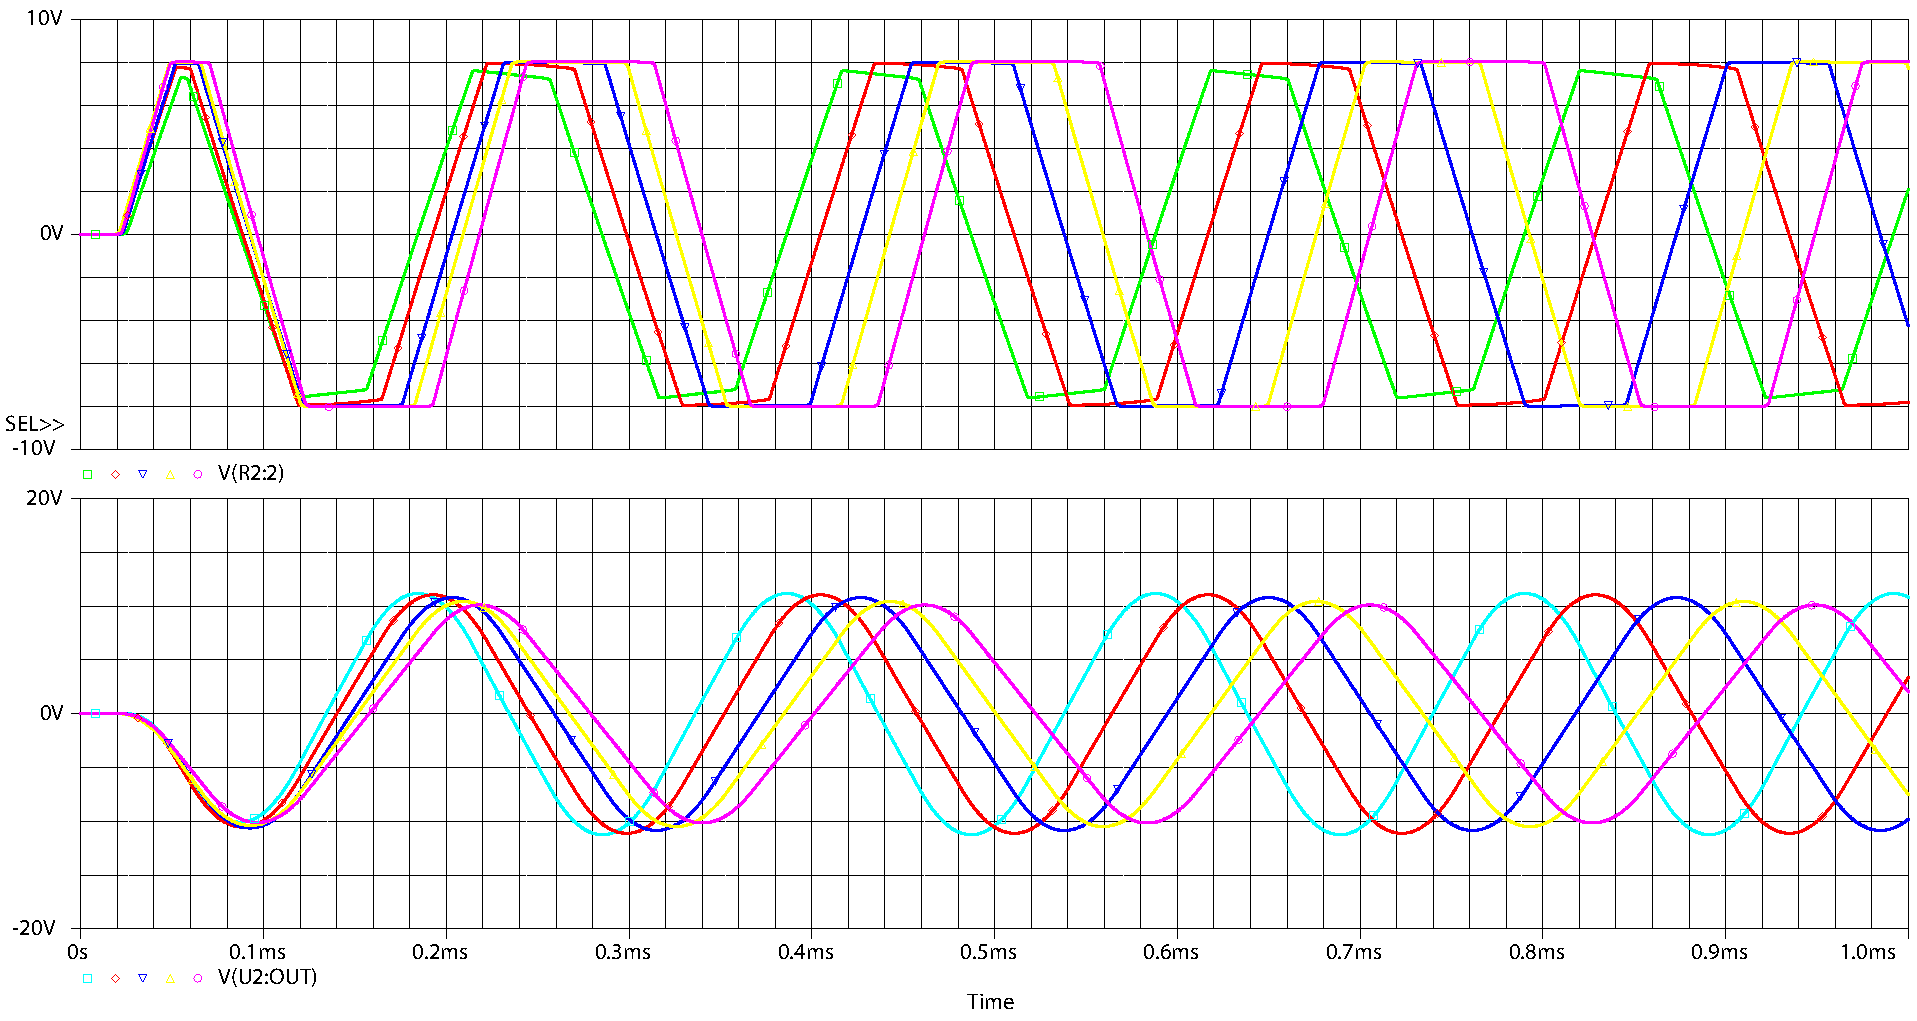
\includegraphics[width=15cm]{spice_01/q5_3.pdf}
		\caption{\textsl{Άνω διάγραμμα}: $v_2$ (\texttt{V(R2:2)}) για $R\in\left\{5,5.75\ldots,8\right\}\kohm$. \textsl{Κάτω διάγραμμα}: $v_{\mathrm{out}}$ (\texttt{V(U2:OUT)}) για $R\in\left\{5,5.75\ldots,8\right\}\kohm$.}
		\label{plot:ask1:q5_3}
	\end{center}
\end{plot_fig}

Η παραμόρφωση γίνεται αισθητή στην κόκκινη κυματομορφή της $v_2$ (\texttt{V(R2:2)}) η οποία αντιστοιχεί σε $R=5.75\kohm$. Επομένως, η ελάχιστη τιμή της $R$ για την οποία δεν παρουσιάζεται παραμόρφωση θεωρείται η $R=6.5\kohm$ και οι κυματομορφές των $v_{\mathrm{out}}$ και $v_2$ για αυτή την  τιμή της $R$ φαίνονται στο διάγραμμα \ref{plot:ask1:q5_4}.

\begin{plot_fig}[H]
	\begin{center}
		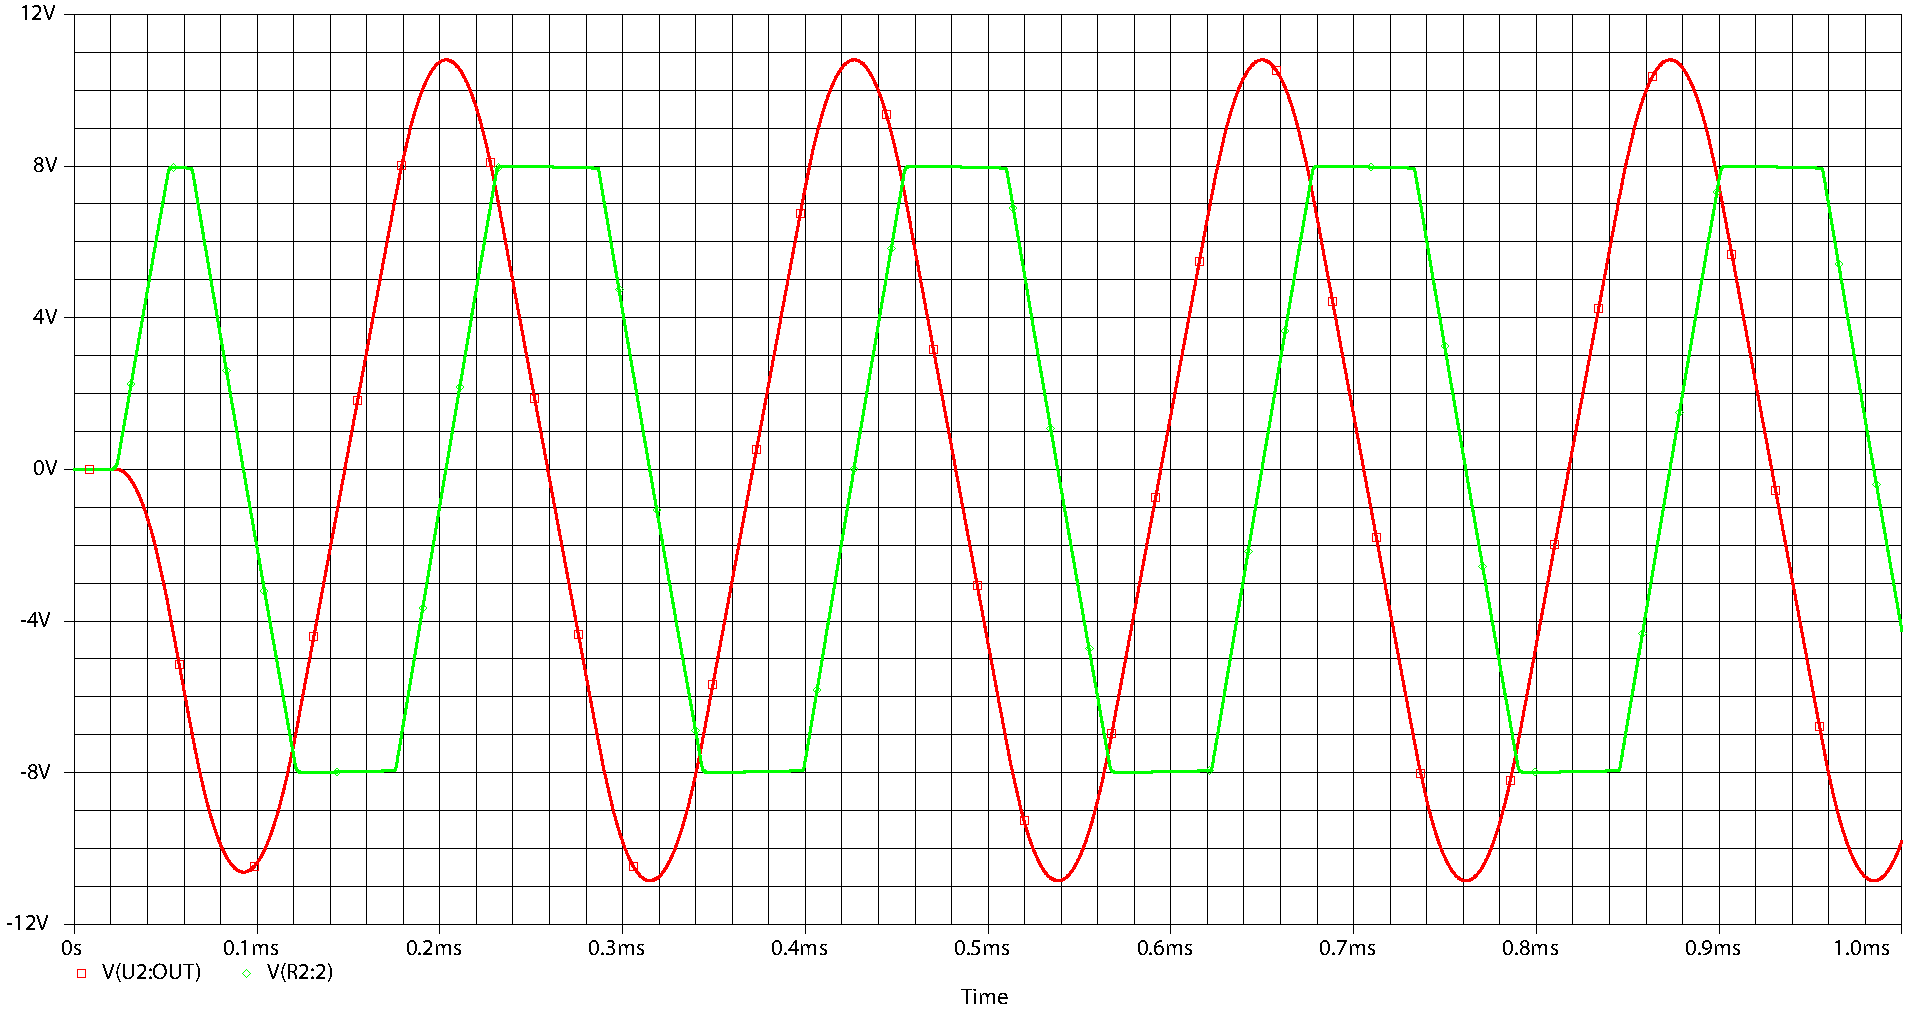
\includegraphics[width=15cm]{spice_01/q5_4.pdf}
		\caption{$v_2$ (\texttt{V(R2:2)}) και $v_{\mathrm{out}}$ (\texttt{V(U2:OUT)}) για $R=6.5\kohm$.}
		\label{plot:ask1:q5_4}
	\end{center}
\end{plot_fig}

Οι περίοδοι των $v_{\mathrm{out}}$ και $v_2$ μετρήθηκαν και βρέθηκαν $T_{\mathrm{out}}=223.285\unit{\micro\second}$ και $T_{2}=223.185\unit{\micro\second}$ αντιστοίχως. Συνεπώς, οι συχνότητες είναι $f_{\mathrm{out}}=4.4786\unit{\kilo\hertz}$ και $f_2=4.4806\unit{\kilo\hertz}$.